\documentclass[a5paper]{article}
\usepackage[a5paper, top=17mm, bottom=17mm, left=17mm, right=17mm]{geometry}
\usepackage[utf8]{inputenc}
\usepackage[T2A,T1]{fontenc}
\usepackage[colorlinks,filecolor=blue,citecolor=green,unicode,pdftex]{hyperref}
\usepackage{cmap}
\usepackage[english,russian]{babel}
\usepackage{amsmath}
\usepackage{amssymb,amsfonts,textcomp}
\usepackage{color}
\usepackage{array}
\usepackage{hhline}
\hypersetup{colorlinks=true, linkcolor=blue, citecolor=blue, filecolor=blue, urlcolor=blue, pdftitle=1, pdfauthor=, pdfsubject=, pdfkeywords=}
\usepackage{graphicx}
\usepackage{indentfirst}
\usepackage{wrapfig}

\sloppy
\pagestyle{plain}

\title{Студенческие проекты по программированию как средство формирования профессиональных навыков у учащихся}

\author{Т.А.Брыксин}
\date{}
\begin{document}

\maketitle
\thispagestyle{empty}

\begin{quote}
\small\noindent
В статье рассматривается проблема формирования практических навыков у студентов университетов, обучающихся по IT-специальностям. Обсуждается идея организации студенческих проектов и летних школ по программированию как средства сближения классического университетского образования и индустрии. Приводится обзор и анализ летних школ и студенческих проектов, проводившихся на базе кафедры системного программирования СПбГУ, обсуждаются трудности в организации подобных мероприятий.
\end{quote}

\section*{Введение} 
Программная инженерия (software engineering,~\cite{swebok}) -- сравнительно молодая и динамично развивающаяся область знаний. В условиях непрерывной эволюции аппаратных платформ, развития разного рода распределенных систем, а также все возрастающего применения вычислительных устройств в различных отраслях промышленности и производства растет потребность в программном обеспечении (ПО).  При этом сами технологии программирования тоже не стоят на месте -- количество языков программирования исчисляется тысячами~\cite{langList}, для многих из них создаются и развиваются различные библиотеки, модули, среды разработки. Для разработки и поддержки современного ПО IT-специалисты должны обладать умениями и навыками работы с самыми современными технологиями программирования (под IT-специалистами в данной статье подразумеваются профессионалы-практики в области программной инженерии, т.е. выпускники специальностей 010503, 010400, 231000 и им подобным). 
 
В настоящее время срок обучения в университете бакалавра составляет три-четыре года, специалиста -- пять лет, последующая магистратура -- еще два, аспирантура -- еще три. Однако 4-6 лет в современной программной инженерии -- это настолько большой срок, что к моменту завершения студентом обучения по специальности существенная часть полученных им практических знаний и навыков теряет актуальность. Причем студенты очень быстро осознают этот факт, и это сильно снижает как их мотивацию к дальнейшей учебе, так и популярность IT-направлений университетов в целом. 

Кроме того, так как за время учебы по IT-специальностям студентов учат чаще всего только  программированию, и чаще всего программированию  какого-то определенного набора задач (например, распространенные структуры данных и применение алгоритмов для работы с ними). При этом курсы по управлению требованиями, менеджменту программных проектов, тестированию и пр., чаще всего преподаваемые на старших курсах, пока еще зачастую не обладают должным качеством и рассматриваются студентами как дополнительная и необязательная информация. Да и как можно научить управлению проектами в учебной среде, изолированной от проблем реальной жизни? Поэтому у студентов складывается впечатление, что работа программиста заключается исключительно в программировании  (т.е. в переводе алгоритмов на машинный язык). Однако еще Ф. Брукс-младший в своей работе ``Мифический человеко-месяц''~\cite{brooks} отмечал, что дополнительные виды деятельности требуют примерно в 3 раза больше ресурсов, чем просто написание этого кода. А задачи интеграции создаваемого ПО с уже существующей инфраструктурой могут увеличить эту цифру еще раза в три. Профессиональные стандарты, разработанные под эгидой Ассоциации предприятий компьютерных информационных технологий (АП КИТ) в 2011 году~\cite{apkit},  отмечают целый ряд ключевых активностей, в которых должен участвовать профессональный программист -- общение с закачиком, работа с требованиями, изучение предметной области и создание сценариев использования продукта, выбор используемых технологий, отладка, тестирование и интеграция разрабатываемых модулей, ведение разного рода документации, ревьюирование кода и документации, получение и анализ численных характеристик проекта и многое другое. Сходные требования к навыкам  выпускаемых из университетов инженерам-программистам предъявляются в ``Рекоммендациях по преподаванию программной инженерии и информатики в университетах''~\cite{curriculum}. 

В университетах традиционными формами передачи знаний  являются практические занятия, лабораторные, курсовые и дипломные работы. Как правило, они слабо связаны с реалиями промышленного программирования. Чтобы идти в ногу со временем и давать студентам актуальные знания и навыки, необходимо тесное сотрудничество с индустрией. Так, можно приглашать практикующих специалистов к преподаванию, организовывать выполнение университетскими лабораториями коммерческих наукоёмких тематических заказов, совершенствовать существующие учебные планы, внедрять новые курсы по актуальным в индустрии темам и и т.п. Однако, перестраивание учебных программ -- процесс небыстрый, а привлечение к преподаванию высококлассных специалистов может потребовать серьезных материальных вложений, в результате чего большинству университетов оказывается удобнее просто не замечать проблемы и придерживаться традиционных подходов к обучению программированию.

Еще одним из способов преодоления разрыва между университетским образованием и реальным промышленным программированием является организация студенческих проектов и летних школ. Данный вид деятельности подразумевает взаимодействие промышленных компаний с университетами и привлечение профессиональных разработчиков с одной стороны и заинтересованных студентов с другой к совместной работе над актуальными задачами в различных областях. Нам кажется, что организация подобных проектов не только представляется хорошим дополнением к перечисленным выше мероприятиям по улучшению процесса обучения программной инженерии, но и является менее затратной для проведения. Например, так как промышленные компании очень заинтересованы в подготовке новых кадров, они часто бывают готовы брать на себя оплату времени своих специалистов, потраченное на работу со студентами. 
 
В данной статье дается обзор летних школ и студенческих проектов, проводимых на кафедре системного программирования Санкт-Петербургского государственного универсистета, обсуждаются трудности в организации подобных мероприятий.

\section{Обзор}

В настоящее время по всему миру организуется большое количество разных школ и практических семинаров (workshops) по информатике и программированию. Примерами таких мероприятий в России могут быть школы, организуемые Microsoft –  Summer School in Software Engineering and Verification~\cite{ms1}, Microsoft Сomputer Vision School~\cite{ms2}, Microsoft Data Structures and Algorithms School~\cite{ms3}). Можно упоминуть также  летние и зимние школы компании Intel~\cite{intel1, intel2, intel3}. Также много мероприятий, нацеленных на круг профессональных программистов,  аспирантов и ученых-исследователей, проводится в европейских университетах, вот некоторые из них. 

\begin{itemize}
  \item Ежегодная летняя школа по программной инженерии LASER, организуемая Швейцарской высшей технической школой Цюриха (ETHZ)~\cite{school1}.  В 2011 году школа была посвящена вопросам верификации программного обеспечения.
  \item Проходящая раз в два года в г. Брага (Португалия) летняя школа, посвященная техникам генерации и трансформаций в программной инженерии~\cite{school2}. В  2011 году школа была совмещенна с семинарами CSXW 2011~\cite{school3} и ITSLE 2011~\cite{school4}. 
  \item Ежегодная международная летняя школа по программной инженерии, организуемая университетом г. Салермо (Италия)~\cite{school5}.
  \item Летняя школа по языкам программирования для параллельных вычислений, проведенная в июне 2011 года Уппсальским университетом (Швеция)~\cite{school6}.
  \item Школа, посвященная вопросам многоядерных архитектур, проходившая в июле 2011 года на базе университета г. Амстердама (Голландия)~\cite{school7}.
  \item Летняя школа по научному и высокопроизводительному программированию в г. Эспоо, Финляндия, проведенная в 2011 году при поддержке организации PRACE (Partnership for Advanced Computing in Europe) и Центра высокопроизводительных вычислений Королевского технологического института Швеции (KTH)~\cite{school8}.
  \item Семинары организации SoSE (Software Systems and Engineering), проводимые для аспирантов и ученых-исследователей финских университетов при поддержке министерства образования Финляндии~\cite{school9}.
  \item Финско-русский проект FRUCT~\cite{school10}, в рамках которого два раза в год проводится научно-практическая конференция и сопутствующие семинары. К участию в этих мероприятиях активно привлекаются студенты и молодые исследователи из России и Финляндии.  
  \item Летние школы университета Аалто, университета г. Турку, Тампере, Гронингена и многие другие.
\end{itemize}

Большой список проведенных за последнее годы международных летних студенческих школ по программной инженерии и информационным технологиям можно найти в~\cite{schoolList}. 

Длительность таких школ обычно составляет от нескольких дней до одной-двух недель. Однако, в основном эти мероприятия имеют преимущественно исследовательскую направленность  и больше по формату похожи на конференции -- организаторы собирают именитых ученых или представителей индустрии, которые делают доклады, проводятся обсуждения и сопутствующие семинары на различные темы. Также возможно выполнение небольших практических заданий для ознакомления с технологиями или инструментами, которым посвящена та или иная школа. Однако в целом практические аспекты имеют второстепенное значение, а большая часть времени посвящается докладам, лекциям и дискуссиям. Для решения задачи комплексного формирования у студентов навыков программной инженерии такие мероприятия подходят плохо, поскольку носят узконаправленный характер, требуют от участников специализированный знаний и мало похожи на  реальные промышленные проекты.

Отдельно стоит упоминуть программу компании Google под названием Google Summer of Code~\cite{google}. В рамках программы каждый год выбирается несколько крупных проектов по разработке свободного программного обеспечения, и студенты, желающие принять участие в этом конкурсе, предлагают свои идеи по доработке этих продуктов. Руководители каждого проекта выбирают наиболее понравившиеся им идеи и организуют их реализацию с участием студентов. Тем из участников, кому удается успешно завершить поставленные задачи и получить положительные рекомендации от менторов, компания Google выплачивает денежную премию. Эта инициатива  кажется нам очень удачной, поскольку действительно позволяет участникам получить опыт программирования в актуальных, развивающихся проектах, учиться у руководителей и перенимать опыт организации открытых проектов. Каждый год все больше и больше студентов проходят отборочный этап.  В 2011 году Google принял в эту программу 1026 студентов из 69 разных стран, что в 2.5 раза больше, чем в 2005 году, когда данная программа стартовала впервые. Однако отбор происходит из многих тысяч желающих со всего мира, и большинству желающих не удается принять участие в этой программе. При наличии подобных мероприятий в рамках отдельных университетов, при тесном сотрудничестве с близлежащими индустриальными компаниями, можно было бы серьезно улучшить подготовку студентов по IT-специальностям.

\section{Опыт СПбГУ}

На протяжении более чем десяти лет при сотрудничестве с ЗАО ``Ланит-Терком''~\cite{tercom} кафедра системного программирования СПбГУ организует студенческие проекты, активно привлекая к сотрудничеству опытных промышленных программистов и инициативных студентов~\cite{gagarsky}. Каждый семестр ЗАО ``Ланит-Терком'' предлагает студентам ряд проектов из различных областей, начиная от встроенных систем и заканчивая Web-системами и мобильными приложениями. Все проекты являются некоммерческими, как правило, с открытым исходным кодом, что позволяет участникам свободно ссылаться на свои проекты в дальнейшем (например, в резюме). Работа студентами ведется дома в свободное время, общение с руководителем осуществляется удаленно, чаще всего посредством электронной почты или с помощью средств мгновенного обмена сообщениями. Для координации работ еженедельно проводятся общие собрания, в начале проекта проводятся дополнительные вводные лекции. Все это позволяет студентам гибко планировать график своего участия в проекте, что важно в свете того, параллельно с участием в проекте студенты учатся в университете. 

К участию приглашаются студенты всех курсов. Однако, как показывает практика, б\textit{о}льшую активность проявляют студенты с первого по третий курс. На наш взгляд, это обусловлено тем, что на старших курсах студенты уже начинают работать параллельно с учебой, и у них не хватает времени на участие в студенческих проектах. 

После завершения семестра проводятся презентации результатов каждого проекта. Стоит отметить, что несколько последних лет проводимые проекты стали проходить в годовом формате. Это обусловлено в первую очередь тем, что при старте проекта студентам часто приходится долго разбираться в новой предметной области, в новых технологиях и языках программирования. При этом в семестровом формате на реальную работу в проекте остается мало времени. 

Как показывает практика, студенческие проекты приносят пользу обеим участвующим сторонам. Для компаний это дополнительная реклама в университетских кругах, возможность заинтересовать молодых программистов и пригласить лучших из них к себе на работу. Для руководителей проектов, являющихся работниками этих компаний, студенческие проекты являются возможностью отработать навыки управления проектом, попробовать себя в роли архитектора, ведущего разработчика или менеджера проекта, отработать построение процесса разработки, опробовать новые идеи и решения, которые по тем или иным причинам не могут быть воплощены в жизнь в рамках обычной деятельности компании и пр. Для студентов же это, в первую очередь, возможность изучить новые для себя языки и технологии, получить опыт работы над нетривиальным проектом, перенять знания и практические навыки у опытных программистов, получить рекомендацию для дальнейшего устройства на работу. 

Однако, несмотря на то, что участники студенческих проектов осваивают многие инженерные практики, принятые в промышленном программировании (например, использование систем контроля версий, организация ночных сборок и тестирования, ревью кода и т.п.), данные проекты слабо напоминают полноценную работу в промышленной компании. Это происходит, в частности, из-за свободного и неинтенсивного графика работы, преимущественно удаленного общения с руководителем, отсутствия внешних заказчиков и т.п.

Для решения части из этих проблем кафедра системного программирования СПбГУ совместно с ЗАО ``Ланит-Терком'', дополнительно к студенческим проектам в последние годы проводит летние школы по программированию. Эти школы проходят во время летних каникул, традиционно начинясь сразу после сессии. Каждому проекту предоставляется аудитория, обрудованная компьютерной техникой, доской, проектором и прочими необходимыми для проведения занятий средствами. Работа происходит в течение одного месяца ориентировочно по 20 рабочих часов в неделю, что соответствует половине ставки профессионального программиста. Руководители каждого из проектов вольны сами выбирать график работы для своих команд – с либо 5 дней в неделю по 4 часа в день, либо 4 дня по 5 часов, возможны также и другие варианты. Все это позволяет сильно поднять интенсивность работ по сравнению со студенческими проектами: студенты проводят каждый день значительное время, работая в команде, постоянно находятся в контексте проекта, не переключаясь на учебу и другие занятия, как это бывает при участии в студпроекте в течение семестра. Сжатость временных сроков также позволяет быстрее получать и анализировать результаты, адекватно оценивать свою производительность и строить выполнимые планы для дальнейшей работы. 

На протяжении последних нескольких лет каждый семестр проводилось от 6 до 10 студенческих проектов (см. рис.~\ref{projects}), в каждом из которых было задействовано от 5 до 20 студентов. На графике также отражены летние школы 2010 и 2011 года, объединившие в себе по 5 и 12 проектов соответственно. Большое число проектов позволило покрыть обширный круг областей от операционных систем реального времени до мобильных приложений, давая студентам возможность выбрать наиболее интересные для них направления.

\begin{figure} [ht]
  \begin{center}
    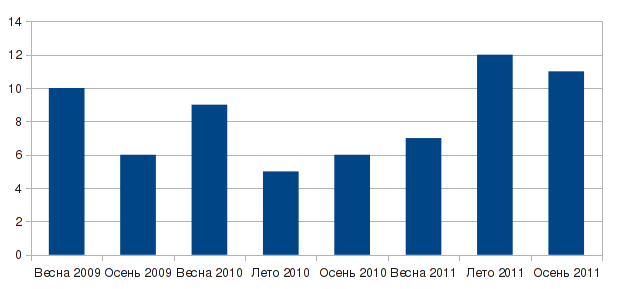
\includegraphics[width=1\textwidth]{01-projects.png}
    \caption{Число студенческих проектов по семестрам, 2009 – 2010 гг.}
    \label{projects}
  \end{center}
\end{figure}

Интересно также то, что в осенние семестры студенческие проекты оказывались менее популярны, чем в весенние. Это объясняется в большей степени тем, что весной для второкурсников происходит распределение по кафедрам, а активным участием в студпроекте можно заработать рекомендацию на интересующую кафедру. 

Сильный всплеск числа летних школ по программированию в 2012 году объясняется тем, что в организации этого мероприятия приняло участие сразу несколько компаний. Так, помимо традиционных проектов от ЗАО “Ланит-Терком”, работа проводилась еще в двух направлениях: разработка дружественных пользовательских интерфейсов и юзабилити (при поддержке лаботатории Sprint и компании Intel), системному программированию и компьютерной безопасности (при поддержке компаний Digital Design, EMC, Лаборатория Касперского, ЦентрИнформ). В этом году три этих направления были объединены в школу системного программирования при кафедре системно программирования СПбГУ. Однако, де-факто они были в значительной степени обособлены. В дальнейшем планируется теснее интегрировать между собой эти и другие летние IT-мероприятия для студентов, проводимые в СПбГУ. 

\section{Проекты}

Остановимся подробнее на проектах, проведенных кафедрой системного программирования СПбГУ в 2010 году при сотрудничестве с ЗАО ``Ланит-Терком''. Большая часть из них была нацелена на изучение популярных сейчас мобильных и Интернет-технологий.

Так, несколько проектов было посвящено мобильной платформе Android. В рамках проекта ``Цена денег'' был разработан виджет, позволяющий отображать текущую ситуацию на различных рынках: российском валютном рынке, рынке цветных металлов и т.п. Другой проект ``Android-GeoCacheing.su'' был посвящен взаимодействию мобильных приложений с Интернет-сервисами, а также программному использованию GPS- приемника и магнитного компаса для реализации навигационных приложений. Работа была организована таким образом, что участники проекта знакомились со всеми этапами промышленной разработки ПО, начиная от создания технического задания и заканчивая выпуском финальной версии и написанием документации. Разработка в этих проектах происходила на языке Java. 

Проект ``iPhoneCF'' также был направлен на разработку ПО в области мобильных платформ. Его целью была создание инструмента для построения распределенных систем, работающих в операционной системе iPhone. Помимо, собственно, технологических вопросов (знакомство с операционными системами Mac OS, iPhone OS, а также языком Objective C и средой разработки Xcode) в данном проекте много внимания уделялось организации процесса разработки: работа велась в соответствии с ``гибкой'' методологией Scrum. В дальнейшем проект был продолжен под названием ``NeuronIOS'' и был посвящен созданию среды для реализации приложений для операционной системы iPhone, использующих аппарат нейронных сетей для обработки и анализа данных.

Проект ``Basis'' ставил своей целью создание среды для разработки php-приложений. Подобный инструментарий должен минимизировать затраты php-программиста на написание типовых управляющих элементов интерфейса и функций, а также предоставить разработчику каркас приложения, в котором разделена логика по обработке запросов, по работе с базой данных и т.п. Работы велись на языке PHP5 с использованием технологи AJAX.

Проект ``News Aggregating Agent'' предполагал создание приложения для социальных сетей, выполняющих просмотр собираемых с различных Интернет-источников новостей с возможностью фильтрации (по каналу, теме и/или дате). В рамках данного проекта студенты знакомились с программными интерфейсами ведущих социальных сетей и учились создавать Web-приложения на языке haXe.

Проект ``BoardGameMaster'' был посвящен другому популярному в наше время типу Интернет-приложений -- многопользовательским онлайн-играм. Задача данного проекта заключалась в разработке Web-сервиса, обеспечивающего возможность реализации любой игры с последовательными действиями игроков (от традиционных шахмат до современных настольных игр). В качестве примера клиентского приложения была разработана электронная версия настольной игры Dominion, разработка которого велась с использованием технологии Flash. Данный студпроект разрабатывался  в течение нескольких семестров.

В рамках проекта ``SUGAR'' студенты занимались созданием приложения для работы с кулинарными рецептами. Данное приложение позволяло по заданному набору продуктов выдать рекомендации, что их них лучше приготовить и как именно, а также подсказывало, что и в каком количестве необходимо дополнительно купить, предоставляя возможность осуществить заказ в Интернет-магазине. Здесь активно использовались технологии компании Miscrosoft -- платформа .NET 3.5-4, Silverlight, SQL Server.

Еще один студенческий проект был направлен на освоение одной из самых популярных платформ разработки Java-приложений -- Eclipse, в том числе технологий работы с XML-документами и одной из самых мощных на сегодняшний день платформы для автоматизированного создания графических редакторов -- Eclipse Graphical Modeling Framework (GMF). В качестве области для экспериментов проводилась разработка средства для создания и управления семейством пользовательской документации программного продукта. 
 
Отдельного упоминания заслуживают проекты Embox~\cite{embox} и QReal~\cite{qreal}, разрабатываемые как свободное программное обеспечение и традиционно предлагаемые в рамках студенческих проектов и летних школ. 

Проект Embox направлен на создание переносимой  и конфигурируемой операционной системы реального времени для нужд встроенных приложений. Данная система применяется на всех стадиях разработки, от проектирования аппаратной части и до создания функционального ПО. Операционная система  запускается на различных процессорных архитектурах, включает в себя сетевой стек, файловую подсистему, частично поддержан стандарт POSIX и многое другое. Проект ведется уже несколько лет и каждый год привлекает много новых студентов, интересующихся внутренним устройством операционных систем.  

Проект QReal посвящен модельно-ориентированному подходу к разработке ПО, в частности, предметно-ориентированному моделированию – созданию metaCASE-системы . В рамка проекта ведется разработка инструментария, позволяющего быстро разрабатывать новые графические языки и визуальные редакторы для них, а также генераторы кода в различные целевые языки, визуальные отладчики и другие полезные для разработки ПО средства. Студенты знакомятся с устройством визуальных языков, а также принимают активное участие в развитии системы QReal. 

\section{Проект QReal}

Рассмотрим некоторые примеры того, как участие в летней школе может способствовать формированию у студентов практических навыков программной инженерии. 

В 2011 году летняя школа в рамках исследовательской группы QReal была посвящена созданию QReal:Robots -- средства визуального программирования роботов Lego Mindstorms NXT 2.0. В настоящее время наблюдается активный рост использования робототехнических конструкторов в школах как средств обучения программированию и робототехнике~\cite{filippov}. Однако, существующие средства программирования таких устройств во многом не устраивают учителей. В частности, некоторые из существующих средств недостаточно функциональны, другие не позволяет наглядно отлаживать создаваемые программы, не имеют возможностей перехода от графического представления программы к текстовому, не до конца переведны на русский язык, а также зачастую небесплатны. При сотрудничестве с кафедрой теоретической кибернетики СПбГУ и ФМЛ №239 г. Санкт-Петербурга было решено разработать отечественное средство программирования данных роботов Lego. 

Проект по разработке такой среды стартовал в январе 2011 года, так что к началу летней школы уже существовал некий прототип, умеющий выполнять базовые операции. Важной особенностью данной школы стало фактическое наличие внешнего заказчика и жестких дедлайнов. В качестве заказчиков выступали заинтересованные в этом программном продукте учителя, которым посредством выступления на тематических конференциях было анонсировано о выпуске бета-версии продукта к началу нового учебного года, т.е. формально через некоторое время после завершения летней школы. Это добавило участником летней школы дополнительной мотивации, поскольку они понимали, что создаваемый ими продукт -- это не учебная разработка, он действительно нужен. Осознание этого факта позволяло студентам более ответственно относиться к ставившимся перед ними задачам.

В случае, когда фактический заказчик отсутствует, его роль может взять на себя руководитель проекта. Однако, это может вызвать дополнительные сложности, поскольку руководителю придется совмещать роли, интересы которых в проекте традиционно конфликтуют -- заказчик хочет как можно больше функциональности за меньший объем ресурсов, а менеджер проекта пытается сокращать объем планируемой функциональности в пользу качества и стабильности проекта в целом. Если же руководитель проекта берет на себя только роль заказчика, управление проектом и организация команды перекладывается на плечи студентов, что в отсутствие у них подобного опыта может стать непосильной задачей.

Возвращаясь к QReal:Robots, кроме реализации новой функциональности, связанной с генерацией по диаграммам кода на языке Си, автоматической прошивкой программы на робота, организации управления робота по USB и т.п., много времени уделялось исправлению имеющихся ошибок и стабилизации имеющегося кода. Данный вид деятельности также очень важен, поскольку, во-первых, стадия развития и поддержки существующего кода присутствует в жизненном цикле любого проекта, а во-вторых, приучает студентов аккуратнее относиться к этапам проектирования и реализации задач, которые перед ними ставятся.

Особую специфику может добавить участие в проекте, разрабатываемом как свободное программное обеспечение (СПО) ~\cite{saratov}. В частности, чувство владения (``feeling of ownership'') кодом продукта у студентов также повышает личную ответственность за реализуемую ими функциональность, что помогает не делать поспешных и необдуманных решений. Стоит отметить, что поначалу некоторых студентов может испугать такая открытость и они будут бояться выкладывать свои изменения в публичный доступ. Однако, как показывает практика, такое поведение наблюдается лишь поначалу, потом студенты привыкают к концепции открытого ПО вплоть до того, что начинают хвастаться своими успехами перед одногруппниками. 

Еще одним полезным видом деятельности, про который нельзя забывать при организации студенческих проектов и летних школ, является практика ревью кода. Зная, что их изменения обязательно будут просмотрены и прокомментированы перед интеграцией в общую кодовую базу, студенты будут стараться программировать аккуратнее. А участие в ревью кода своих коллег позволяет им учиться на чужих ошибках, пытаясь подобным образом анализировать свои решения в дальнейшем. Ревью кода стоит проводить на регулярной основе, например, один или два раза в неделю для летних школ и, скажем, раз в неделю для студенческих проектов в течение семестра.

Другим важным фактором успешности проведения подобных проектов наряду с открытостью является наличие возможности у студента увидеть результат своей работы. В частности, участие в разработке крупных программных систем возможно либо при наличии уже готового прототипа, либо при участии в разработке какого-то уже существующего открытого проекта (по аналогии с Google Summer of Code). Но для студентов это может быть сложно из-за языкового барьера и/или отсутствия опыта участия в крупных открытых проектах. В таком случае руководителю нужно быть хорошо знакомым с разрабатываемым проектом и брать часть коммуникаций с основной командой разработчиков на себя.

\section{Выводы} 

Традиционное университетское образование направлено в первую очередь не на получение практических навыков, а на формирование особого образа мышления студентов -- умения искать и анализировать информацию, не просто решать известные задачи, а находить новые пути решения. Для обучения по специальностям, связанным с программной инженерией, это имеет свои плюсы и минусы: с одной стороны, выпускник классического университета получает фундаментальную теоретическую подготовку для работы в своей области -- знает основные алгоритмы и структуры данных, языки программирования, технологии и подходы к разработке ПО и т.д. С другой стороны, на лицо явный недостаток практических навыков, и это хорошо понимают в промышленных компаниях -- к большинству из открытых в индустрии вакансий ставится требованием наличие нескольких лет опыта работы по специальности. Осознавая это, студенты IT-специальностей, начиная с третьего-четвертого курса, уже пытаются устраиваться на работу стажерами. Но очень часто это приводит тому, что у них остается очень мало времени на учебу. В результате уровень получаемого выпускниками образования снижается.

Решать эту проблему, безусловно, нужно. А так как речь идет о практической дисциплине, то большую роль в формировании профессиональных навыков программной инженерии играет передача опыта, описание типичных ошибок и практик, зарекомендовавших себя в индустрии, примеры выполнения реальных проектов и т.п. Ведь нельзя стать хорошим программистом, только лишь читая книги, сидя в лекционном зале или в компьютерном классе. 

Одной из форм получения реального промышленного опыта наиболее гармоничным образом является совместная (промышленные компании и университеты) организация студенческих проектов и летних школ. Участвуя в подобных проектах, студенты не только повышают свои навыки программирования, но и знакомятся с полезными инженерными практиками, которые помогут им по завершении обучения быть полноценными специалистами в области программной инженерии. Так, студенты учатся взаимодействовать в команде, использовать системы версионного контроля для кода и документации, выявлять и анализировать требования, оценивать и планировать задачи, участвовать в ревью кода, архитектуры, документации и других артефактов проекта. Кроме того, в рамках студпроекта студент может подготовить курсовую работу, а также получить рекомендацию для устройства на работу в компанию, которую представляет руководитель проекта. 

В настоящее время при организации студенческих проектов и летних школ можно столкнуться с множеством сложностей на самых разных уровнях. 

\begin{itemize}
 \item Нужно организовать финансирование. Идеальным является совместные финансовые вложения бизнес-компаний и университетов. Также можно привлекать различные гранты, фонды на региональном, федеральном и международном уровнях. 
 \item Необходимо уладить все формальные вопросы с университетом, включая организацию подходящих для работы помещений. Сложность и трудоемкость этой деятельности нельзя приуменьшать, так как российские университеты все строже регламентируют свою деятельность, и необходимо получить множество различных разрешений и одобрений, попасть в различные планы официальных мероприятий и т.д. 
 \item Нужно привлечь заинтересованных в IT-компаниях специалистов для руководства проектами. При  этом идеальной является ситуация, когда специалистам в университете интересная  тематика того или иного студенческого проекта, и они помогают наладить долгосрочное сотрудничество с промышленной компанией и гармоничный учебный процесс для студентов.  
 \item Необходимо также подобрать подходящие задачи, которые заинтересуют студентов и будут актуальными для современной программной инженерии, а также будут им посильны. 
 \item Наконец,  требуется разработать методики проведения студенческих проектов и летних школ, которые позволят делать их максимально эффективными – при этом есть много нюансов, которые будут отличаться в каждом конкретном случае.  
 \item Если студенческая школа проводится регулярно, то ей нужен хороший сайт, что крайне полезно как для привлечения студентов, компаний-участников и финансирования. 
\end{itemize}
  
Как показывает опыт проведения таких мероприятий на базе кафедры системного программирования СПбГУ, для студентов опыт участия в них крайне полезен. И растущее с каждым годом число проводимых по всему миру летних школ по программированию и информатике лишь подтверждает это.

\begin{thebibliography}{9001}
  \bibitem{ms1} Summer School in Software Engineering and Verification, Moscow, 2011, \url{http://research.microsoft.com/en-us/um/redmond/events/sssev2011/}
  \bibitem{ms2} Microsoft Сomputer Vision School, Moscow, 2011, \url{http://summerschool2011.graphicon.ru/en}
  \bibitem{ms3} Microsoft Data Structures and Algorithms School, St.Petersburg, 2010, \url{http://logic.pdmi.ras.ru/midas/en/about}
  \bibitem{intel1} Летняя школа Intel 2010, \url{http://software.intel.com/ru-ru/articles/summer-school-2010-main/}
  \bibitem{intel2} Летняя школа Intel 2011, \url{http://software.intel.com/ru-ru/articles/summer-school-2011/}
  \bibitem{intel3} Студенческие школы компании Intel, \url{http://www.intel.com/cd/corporate/education/emea/rus/highered/student/398668.htm}
  \bibitem{school1} 8th LASER Summer School on Software Engineering, о. Эльба, Италия, 2011, \url{http://laser.inf.ethz.ch/2011/}
  \bibitem{school2} 4th Summer School on Generative and Transformational Techniques in Software Engineeringh, Брага, Португалия, 2011,  \url{http://gttse.wikidot.com/}
  \bibitem{school3} Coupled Software Transformations Workshop, Брага, Португалия, 2011, \url{http://www.di.univaq.it/CSXW2011/}
  \bibitem{school4} Industry Track of Software Language Engineering, Брага, Португалия, 2011, \url{http://planet-sl.org/itsle2011/index.php?option=com_content&view=article&id=128&Itemid=169}
  \bibitem{school5} 8th International Summer School on Software Engineering, Салермо, Италия, 2011, \url{http://www.sesa.dmi.unisa.it/seschool/}
  \bibitem{school6} Programming Languages for Concurrent \& Parallel Computing, Стокгольм, Швеция, 2011, \url{http://www.it.uu.se/research/upmarc/events/SS2011/Start.html}
  \bibitem{school7} Школа, посвященная вопросам многоядерных архитектур, Амстердам, Голландия, 2011, \url{http://www.multimoore.nl/}
  \bibitem{schoolList} Список некоторых летних школ с 1998 по 2011 по IT, \url{http://user.it.uu.se/~bengt/Info/summer-schools.shtml}
  \bibitem{school8} PRACE Summer School, Эспоо, Финляндия, 2011, \url{http://www.csc.fi/english/csc/courses/archive/summerschool2011}
  \bibitem{school9} Семинары компании SoSE, Саариселка, Финляндия, \url{http://www.cs.tut.fi/~sose/index_files/Page1211.htm}
  \bibitem{school10} Finnish-Russian University Cooperation in Telecommunications, \url{http://www.fruct.org/}
  \bibitem{langList} HOPL: an Interactive Roster of Programming Languages,  \url{http://hopl.murdoch.edu.au/}
  \bibitem{brooks} Ф. Брукс. Мифический человеко-месяц или Как создаются программные системы, Символ-Плюс, СПб., 2011
  \bibitem{apkit} Квалификационные требования (профессиональный стандарт) в области информационных технологий по специальности ``Программист'', \url{http://apkit.ru/files/programer.doc}
  \bibitem{curriculum} Рекоммендациях по преподаванию программной инженерии и информатики в университетах, \url{http://www.intuit.ru/research/se2004.pdf}
  \bibitem{swebok} Guide to the Software Engineering Body of Knowledge (SWEBOK), \url{http://www.computer.org/portal/web/swebok}
  \bibitem{google} Google Summer of Code, \url{http://code.google.com/intl/ru-RU/soc/}
  \bibitem{gagarsky} Р.К Гагарский. Программа подготовки специалистов в IT-компании // Системное программирование. Вып. 3. СПб.: Изд-во СПбГУ. 2008, С. 141-156
  \bibitem{tercom} ЗАО «Ланит-Терком», \url{www.lanit-trecom.ru}
  \bibitem{embox} Проект Embox, \url{http://code.google.com/p/embox/}
  \bibitem{qreal} Проект QReal, \url{qreal.ru}
  \bibitem{filippov} С.А. Филиппов. Робототехника для детей и родителей, Наука, Москва, 2011
  \bibitem{saratov} Я.А. Кириленко. Разработка свободного программного обеспечения для школ как средство обучения программной инженерии // Материалы IX Всероссийской конференции «Преподавание информационных технологий в Российской Федерации». Саратов. 2011
\end{thebibliography}

\end{document}